% Fig 3.14 ESR spectrometer: microwave source -> waveguide -> cavity with sample,
% between two hatched magnet pole pieces (45 deg section hatching).
\documentclass[tikz,border=5pt]{standalone}
\usetikzlibrary{arrows.meta,patterns}
\usepackage{amsmath}
\usepackage{bm}
\usepackage{fontspec}
\setmainfont{Times New Roman}
\begin{document}
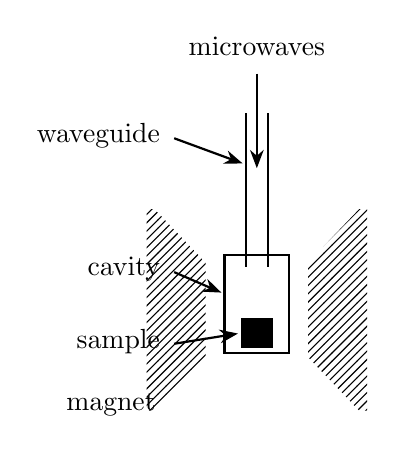
\begin{tikzpicture}[line width=0.8pt,>=Stealth]
% ---------- top: microwaves ----------
\node at (2.6,5.25) {microwaves};
\draw[->] (2.6,4.90) -- (2.6,3.70);
% waveguide (two vertical lines, running into the cavity)
\draw (2.46,4.40) -- (2.46,2.45);
\draw (2.74,4.40) -- (2.74,2.45);
% ---------- cavity ----------
\draw (2.19,2.60) rectangle (3.01,1.35);
% sample (black block on cavity floor)
\fill (2.40,1.42) rectangle (2.80,1.80);
% ---------- magnet pole pieces (hatched) ----------
\fill[pattern=north east lines] (1.20,3.18) -- (1.30,3.18) -- (1.95,2.50)
      -- (1.95,1.30) -- (1.30,0.62) -- (1.20,0.62) -- cycle;
\fill[pattern=north east lines] (4.00,3.18) -- (3.90,3.18) -- (3.25,2.50)
      -- (3.25,1.30) -- (3.90,0.62) -- (4.00,0.62) -- cycle;
% ---------- labels with leaders ----------
\node[anchor=east] at (1.50,4.12) {waveguide};
\draw[->] (1.55,4.08) -- (2.42,3.76);
\node[anchor=east] at (1.50,2.42) {cavity};
\draw[->] (1.55,2.38) -- (2.15,2.12);
\node[anchor=east] at (1.50,1.50) {sample};
\draw[->] (1.55,1.47) -- (2.36,1.60);
\node[anchor=west] at (0.05,0.70) {magnet};
\end{tikzpicture}
\end{document}
